% !TEX TS-program = pdflatex
% !TEX encoding = UTF-8 Unicode

% This is a simple template for a LaTeX document using the "article" class.
% See "book", "report", "letter" for other types of document.

\documentclass[11pt]{article} % use larger type; default would be 10pt

\usepackage[utf8]{inputenc} % set input encoding (not needed with XeLaTeX)

%%% Examples of Article customizations
% These packages are optional, depending whether you want the features they provide.
% See the LaTeX Companion or other references for full information.

%%% PAGE DIMENSIONS
\usepackage{geometry} % to change the page dimensions
\geometry{a4paper} % or letterpaper (US) or a5paper or....
% \geometry{margin=2in} % for example, change the margins to 2 inches all round
% \geometry{landscape} % set up the page for landscape
%   read geometry.pdf for detailed page layout information

\usepackage{graphicx} % support the \includegraphics command and options

% \usepackage[parfill]{parskip} % Activate to begin paragraphs with an empty line rather than an indent

%%% PACKAGES
\usepackage{booktabs} % for much better looking tables
\usepackage{array} % for better arrays (eg matrices) in maths
%\usepackage{paralist} % very flexible & customisable lists (eg. enumerate/itemize, etc.)
\usepackage{verbatim} % adds environment for commenting out blocks of text & for better verbatim
\usepackage{subfig} % make it possible to include more than one captioned figure/table in a single float
% These packages are all incorporated in the memoir class to one degree or another...

%%% HEADERS & FOOTERS
\usepackage{fancyhdr} % This should be set AFTER setting up the page geometry
\pagestyle{fancy} % options: empty , plain , fancy
\renewcommand{\headrulewidth}{0pt} % customise the layout...
\lhead{}\chead{}\rhead{}
\lfoot{}\cfoot{\thepage}\rfoot{}

%%% SECTION TITLE APPEARANCE
\usepackage{sectsty}
\allsectionsfont{\sffamily\mdseries\upshape} % (See the fntguide.pdf for font help)
% (This matches ConTeXt defaults)

%%% ToC (table of contents) APPEARANCE
\usepackage[nottoc,notlof,notlot]{tocbibind} % Put the bibliography in the ToC
\usepackage[titles,subfigure]{tocloft} % Alter the style of the Table of Contents
\renewcommand{\cftsecfont}{\rmfamily\mdseries\upshape}
\renewcommand{\cftsecpagefont}{\rmfamily\mdseries\upshape} % No bold!

%%% END Article customizations

\usepackage[spanish]{babel}
\usepackage{listings} 

%%% The "real" document content comes below...

\title{Investigación de Lenguajes - Scilab}
\author{Gabriel Aumala, Wilson Enriquez}
%\date{} % Activate to display a given date or no date (if empty),
         % otherwise the current date is printed 

\begin{document}
\maketitle
%\tableofcontents % No hace falta un TOC en un artículo corto

\section{Introducción}
Interpretar nuestras ideas matemáticas no es una tarea sencilla para muchas personas, mucho menos para una computadora. Scilab es un lenguaje de programación de alto nivel que se creó para servir de intérprete a la hora de necesitar la ayuda de una computadora para realizar cálculos científicos complicados.  Creado en Enero de 1994, Scilab contiene cientos de funciones matemáticas aplicadas comúnmente en las ciencias junto a las estructuras de datos y gráficos en 2D y 3D encontrados en un lenguaje de alto nivel. Muchos cálculos rudimentarios pueden ser resueltos en Scilab con pocas líneas de código, a diferencia de otros lenguajes que podrían necesitar funciones y librerías adicionales para el mismo problema. En la actualidad, Scilab es usado ampliamente por instituciones tanto de educación secundaria como de educación superior para enseñar varias asignaturas necesarias para la ingeniería y las ciencias matemáticas. Scilab es un software fácil de instalar, gratuito y de código abierto ya que está financiado por Scilab Enterprises. 

\begin{figure}[h]
  \centering
    
\includegraphics{logosci}
  \caption{Logo oficial de Scilab}
  \label{fig:ejemplo}
\end{figure}

\section{Características}
Scilab se caracteriza por tener una amplia gama de herramientas para el manejo de cálculos matemáticos. Posee un nivel de programacción alto permitiendo el acceso hacia estructuras de datos avanzadas, gráfico de funciones en 2D y 3D, manejo de funciones y más.
Profundizando en sus funciones matemáticas, scilab posee herramientas para todas sus ramas como:
\\%
- Ecuaciones Diferenciales.
\\%
- Gráficas de funciones en 2D y 3D.
\\%
- Optimización.
\\%
- Estadísticas.
\\%
- Proceso de Señales.
\section{Historia}
La Historia de Scilab comienza en los años 80', con Blaise, un CACSD (por sus siglas en inglés, diseño asistido de control computarizado) creado en IRIA (Instituto francés para la investigación en Ciencias Computacionales Y Control) y desarrollado principalmente por Francois Delebeque y Serge Steer con el propósito de proveer una herramienta en control automático para investigadores.
\\%
A inicios de los años 90', el programa ya se llamó 'Scilab' y fue luego desarrollado por Inria dentro del Scilab Group compuesto por los 6 siguientes investigadores: Jean-Philippe, François Delebecque, Claude Gomez, Maurice Goursat, Ramine Nikoukhah y Serge Steer.
\\%
Luego se empezó a distribuir Scilab como un software libre. Scilab 1.1, la primera versión lanzada fue colocada en un sitio anónimo el 2 de Enero de 1994. El grupo Scilab, en conjunto con desarrolladores externos, desarrolló Scilab hasta el termino del 2002 con la versión 2.7.
\\%
A inicios del 2003, tomando en cuenta el incremeto de descargas y uso de la gente, y para asegurar su futuro, desarrollo, mantenimiento, soporte y promoción, INRIA decidió crear el Consorcio Scilab  con el soporte de compañias organizaciones académicas.
\\%
Naturalmente, el consorcio Scilab integro a la cadena de investigación Digiteo en el 2008, para proveer el ambiente apropiado para el software. Scilab ha sido desarrollado, mantenido y promovido desde esta unión en el 2008. 
\\%
Scilab Enterprises es fundada in junio del 2010 con el soporte de Inria, para garantizar el futuro de Scilab. Scilab Enterprises ha tomado completamente la carga de la edición y desarrollo de Scilab desde Julio del 2012.
\section{Tutorial de Instalación}

1.	Comenzamos entrando a la página web de Scilab usando la URL: http://www.scilab.org/ como podemos observar en la figura 2.
\\%
\begin{figure}[!h]
  \centering
    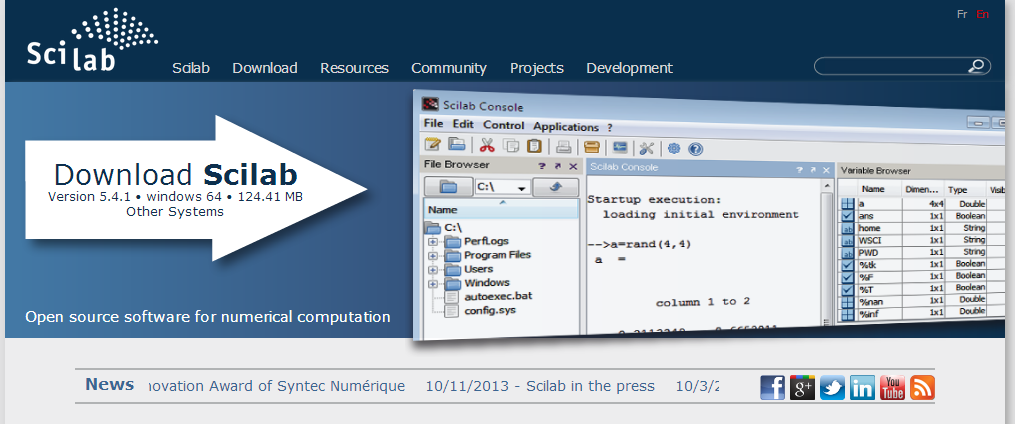
\includegraphics[scale=0.5]{Captura1}
  \caption{Paso 1: Página web de Scilab y link de descarga.}
  \label{fig:paso1}
\end{figure}
\\%

2.	Hacemos click en la flecha que dice “Download Scilab” y procedemos a guardar el instalador en nuestro ordenador.
\\%

3.	Procedemos a abrir el instalador. En la figura 3, podemos observar la ventana que aparece luego de abrirlo.
\\%
\begin{figure}[!h]
  \centering
    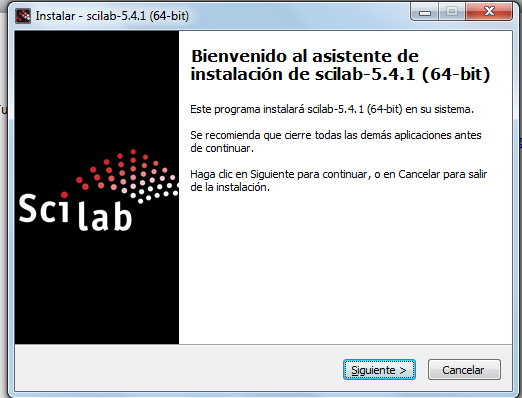
\includegraphics[scale=0.5]{Captura2}
  \caption{Paso 2: Abriendo el instalador}
  \label{fig:paso2}
\end{figure}
\\%

4.	Seleccionamos siguiente, luego aceptamos el acuerdo de licencia y elegimos siguiente. Como se ve en la figura 4.
\\%
\begin{figure}[!h]
  \centering
    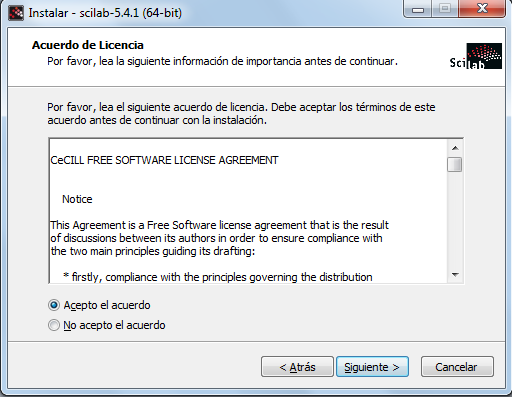
\includegraphics[scale=0.5]{Captura3}
  \caption{Paso 3: Acuerdo de licencia.}
  \label{fig:paso3}
\end{figure}
\\%

5.	Elegimos la carpeta de destino donde se desea instalar Scilab y hacemos click en siguiente, como se observa en la figura 5.
\\%
\begin{figure}[!h]
  \centering
    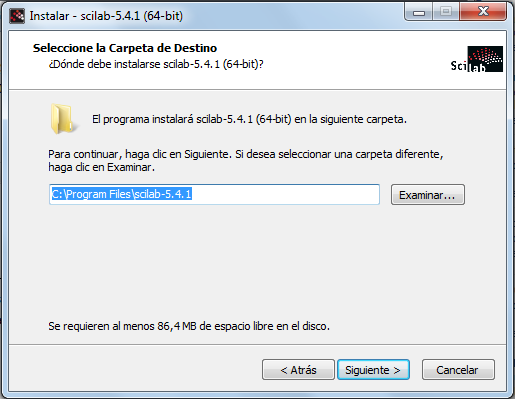
\includegraphics[scale=0.5]{Captura4}
  \caption{Paso 4: Seleccionando carpeta de destino.}
  \label{fig:paso4}
\end{figure}
\\%

6.	Elegimos “Installation (Default)” y escogemos siguiente. En la figura 6 podemos observar las opciones que se presentan.
\\%
\begin{figure}[!h]
  \centering
    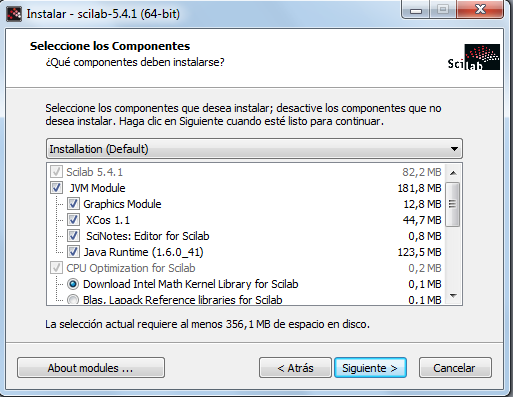
\includegraphics[scale=0.5]{Captura5}
  \caption{Paso 5: Seleccionando el tipo de instalación.}
  \label{fig:paso5}
\end{figure}
\\%

7.	Seleccionamos los iconos de acceso directo que deseamos agregar y damos click en siguiente. 
	En la figura 7 podemos ver los accesos directos que se pueden generar.
\\%
\begin{figure}[!h]
  \centering
    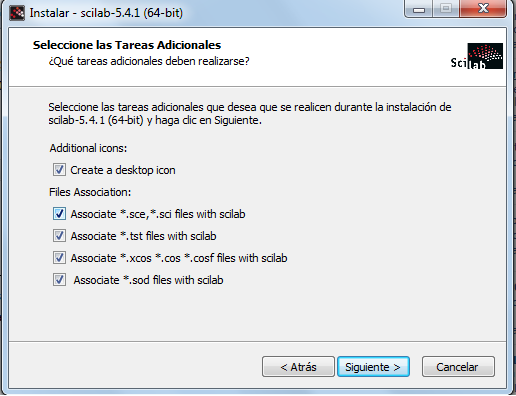
\includegraphics[scale=0.5]{Captura6}
  \caption{Paso 6: Seleccionando accesos directos a Scilab.}
  \label{fig:paso6}
\end{figure}
\\%

8.	Procedemos a instalar Scilab.
\\%

\section{Hola Mundo y otros Programas Introductorios}


Aunque Scilab está orientado a las matemáticas, imprimir por pantalla mensajes de texto es muy sencillo. Esto se puede apreciar en el listing 1:
\lstset{language=Scilab}          % Set your language (you can change the language for each code-block optionally)
\begin{lstlisting}[caption= Código escrito en Scilab para imprimir por pantalla "Hola Mundo!", label=amb, frame=single]  % Start your code-block

disp('Hola Mundo!')
\end{lstlisting}



\end{document}